\chapter{Modelo de Jaynes-Cummings}
\label{ch3_jcm}


%CAMBIAR ESTO PARA PERSONALIZARLO A MI GUSTO
\pagestyle{fancy}
\fancyhf{}
\fancyhead[LE]{\nouppercase{\rightmark\hfill}}
\fancyhead[RO]{\nouppercase{\leftmark\hfill}}
\fancyfoot[LE,RO]{\hfill\thepage\hfill}

En este capítulo se analizará en profundidad el modelo de Jaynes-Cummings (JC), abordando el problema tanto desde un lado te\'orico, como computacional, necesario para resolver posteriormente la din\'amica en sistemas abiertos. Siguiendo los pasos del trabajo \cite{TesisViotti}, se trabajar\'a en el modelo de un átomo en una cavidad, se analizar\'an los casos importantes, y se explicará la din\'amica del problema. Esto resulta importante para comprender conceptualmente cómo interact\'uan fundamentalmente la materia y la luz, y nos sirve para lograr buena intuici\'on del problema de dos átomos. También se ver\'a la influencia del entorno sobre la cavidad, permitiendo pérdidas (o absorci\'on) de fotones, y el bombeo coherente que puede excitar espontáneamente al átomo.  
También se discutirán resultados conocidos sobre la fase geométrica para el modelo de JC disipativo. Finalmente, se extiende el trabajo para considerar un medio no lineal. Se consideran los efectos de las no linealidades sobre las cantidades estudiadas previamente.
\newline

\section{Modelo y aproximaciones}
El modelo de JC consiste en describir la interacción entre la materia y la luz de manera cuántica. El experimento más sencillo consta de un átomo de dos niveles atrapado en una cavidad. La simpleza del modelo surge de las aproximaciones e hipótesis que se hacen; en primer lugar, el campo electromagnético dentro de la cavidad puede, en principio, tener infinitos modos, pero para simplificar se considera solo un modo. 
Entonces el Hamiltoniano que describe el problema es ($\hbar = 1$)

\begin{equation}\label{ec3:hamiltoniano inicial}
\begin{aligned}
    \hat H & = \hat H_A + \hat H_C + \hat H_{int},  \\
    \hat H_A &= \omega \frac{\hat \sigma_z}{2}, \\
    \hat H_C &= \epsilon \hat a^\dagger\hat a = \epsilon \hat n, \\
    \hat H_{int} &= -i g (\hat\sigma_-+\hat \sigma_+)(\hat a - \hat a^\dagger),
\end{aligned}
\end{equation}
donde $\epsilon$ y $\omega$ son las frecuencias naturales de la cavidad y del átomo respectivamente. Los operadores $\hat a$ y $\hat a^\dagger$ son los operadores de aniquilaci\'on y creaci\'on fot\'onicos de la cavidad; $\hat n =a^\dagger a$ es el operador de n\'umero de la cavidad, y $\hat \sigma_z$ es el operador de Pauli del átomo de dos niveles. Los estados del átomo de dos niveles los llamamos $\ket{g}$ y $\ket{e}$ como estados \textit{ground} y excitado respectivamente, y con esta notación los operadores $\hat\sigma_\pm = (\hat\sigma_x\pm i\hat\sigma_y)/2$ son los operadores de subida y bajada atómicos. Con esto en mente, el acoplamiento entre el átomo y la cavidad es mediado por la intensidad $g$. Este es el modelo de Rabi, para arribar al modelo de Jaynes-Cummings hay que simplificar la interacción. Lo que se hace es usar la representaci\'on de interacci\'on en donde se encuentran dos frecuencias: una que se considera \textit{rotante} y es la diferencia entre las frecuencias características $\epsilon-\omega$, y la otra frecuencia es la suma $\epsilon+\omega$. La aproximación de onda rotante vale cuando las frecuencias son similares ($\epsilon\sim\omega$), y consiste en despreciar la dinámica de los términos contrarrotantes ya que oscilan muy rápidamente en comparación con los términos rotantes. Luego, se puede promediar los efectos de los términos rápidos. Entonces al aplicar esta aproximación, justificada cuando $\epsilon\sim\omega$ y $g \ll \epsilon,\omega$ se obtiene el Hamiltoniano de JC \cite{JCoriginal}
\begin{equation}
    \hat H_{JC}=\epsilon \hat a^\dagger \hat a + \frac{\omega}{2} \hat\sigma_z + g(\hat a^\dagger\hat\sigma_-+\hat a\hat\sigma_+).
\end{equation} 
La interpretaci\'on de la interacci\'on en este caso es clara: las dos opciones son que el átomo suba un nivel de energ\'ia y en consecuencia la cavidad pierda un fot\'on, o que el átomo baje un nivel, y la cavidad gane una excitaci\'on. Este Hamiltoniano conserva el n\'umero total de excitaciones $\hat N= \hat n + \hat \sigma$. En este momento es usual aplicar una transformación unitaria $K=\exp{-i\omega t(\hat a ^\dagger \hat a + \hat \sigma_z/2)}$ sobre el Hamiltoniano y así se obtiene
\begin{equation}\label{ec3:hamiltoniano jcm}
    \hat H=\frac{\Delta}{2}\hat\sigma_z+g(\hat a^\dagger \hat\sigma_-+\hat a \hat\sigma_+),
\end{equation} 
donde $\Delta = \epsilon - \omega$ es la desintonía o \textit{detunning} entre las frecuencias de la cavidad y el átomo. El experimento más estudiado de este modelo es un átomo de Rydberg atrapado en una cavidad \cite{Haroche2006}. Como el Hamiltoniano conserva la cantidad de excitaciones es oportuno agrupar los estados en funci\'on de la cantidad de excitaciones: $\{\ket{g,n},\ket{e,n-1}\}$. En esta base el Hamiltoniano se diagonaliza por bloques, donde los elementos de matriz entre estados con diferente cantidad de excitaciones está dado formalmente por
\begin{align*}
    [\hat H,\hat N]=0 \implies & \bra{N'}\hat H \hat N \ket{N} = \bra{N'}\hat N \hat H \ket{N} \\
    & N \bra{N'}\hat H  \ket{N} = N' \bra{N'}\hat H \ket{N} \\
    & \implies \bra{N'}\hat H \ket{N} = \begin{cases}
        0 \text{ , si } N' \neq N \\
        \bra{N}\hat H \ket{N} \text{ , si } N'=N
    \end{cases}
\end{align*}
donde $\ket{N}$ es un estado con $N$ excitaciones totales. Entonces, para resolver el problema solo se tiene que considerar el subespacio de 2x2 de n excitaciones, cuyo Hamiltoniano es
\begin{equation}
    H_n=\begin{pmatrix}
        -\frac{\Delta}{2} & g \sqrt{n} \\
        g \sqrt{n} & \frac{\Delta}{2} 
    \end{pmatrix}.
\end{equation}
Se resuelve el problema de autovalores y autovectores y se obtiene:
\begin{equation}
    \begin{aligned}
        \ket{\psi^n_-} & = \cos \frac{\theta_n}{2}\ket{g,n}-\sin \frac{\theta_n}{2}\ket{e,n-1} \\
        \ket{\psi^n_+} & = \sin \frac{\theta_n}{2}\ket{g,n}+\cos \frac{\theta_n}{2}\ket{e,n-1}        
    \end{aligned}
\end{equation}
con $E_{\pm}^n=\pm \frac{\Omega_n}{2}$ las autoenergias y $\Omega_n=\sqrt{\Delta^2+4g^2n}$ la frecuencia de Rabi del sistema, $\cos \theta_n=\frac{\Delta}{\Omega_n}$ modulando la superposici\'on de estados. 
\begin{figure}
    \centering
    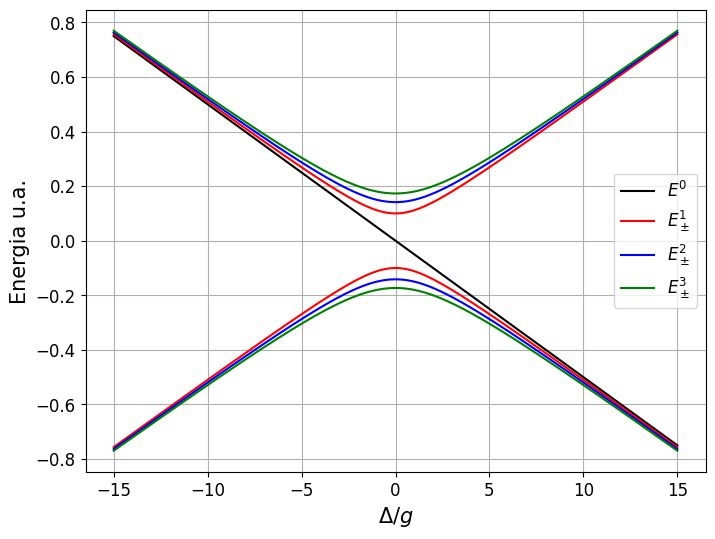
\includegraphics[width=0.7\textwidth]{figuras/ch3/relacion energia detunning jcm simple.png}
    \caption{Relaci\'on energ\'ia detunning para el modelo de Jaynes-Cummings. La diferencia de energ\'ia entre los estados de un mismo nivel para $\Delta=0$ es $2g\sqrt{n}$.}
    \label{fig:relación energia detunning jcm1}
\end{figure}
En la Figura \ref{fig:relación energia detunning jcm1} se observan las curvas de energ\'ia en funci\'on del detunning para diferentes niveles. Lo primero que se tiene que observar es que en el caso resonante, es decir $\Delta=0$, los autoestados del sistema son los estados máximamente entrelazados de Bell
\begin{equation}
    \ket{\psi_\pm^n}=\frac{1}{\sqrt{2}}(\ket{gn}\pm\ket{e,n-1}), 
\end{equation} 
y la diferencia de energ\'ia entre los autoestados es $\Delta E^n =E^n_+-E^n_-=2g\sqrt{n}$. En el caso muy lejos de resonancia se puede asumir que $\Delta \gg g $, y entonces los autoestados coinciden con los estados de la base, 
\begin{equation}
    \begin{aligned}
        \ket{\psi^n_+}=\ket{e,n-1} \\
        \ket{\psi^n_-}=\ket{g,n}.
    \end{aligned}
\end{equation}
Ac\'a hay una sutileza, y es que si $\Delta>0$, entonces $\ket{e,n-1}$ es el estado de mayor energ\'ia y la notaci\'on coincide con la energ\'ia, pero si $\Delta<0$ entonces el estado $\ket{\psi^n_+}$ es el estado de menor energ\'ia. 
Un efecto interesante es que en el caso de alta desinton\'ia, se puede calcular la diferencia entre la energía del autoestado exacto del Hamiltoniano $\ket{\psi_\pm^n}$ y la energía asintótica a la que tiende, que es la energía de los estados de la base $\ket{g,n},\ket{e,n-1}$:
\begin{equation}
    \begin{aligned}
        \Delta E_{e,n-1}=E_+^n-E^{(0)}_{e,n-1}=\frac{g^2}{\Delta}(n+1), \\
        \Delta E_{g,n}=E_-^n-E^{(0)}_{g,n}=-\frac{g^2}{\Delta}(n+1).
    \end{aligned}
\end{equation}
El resultado importante de esta diferencia de energías es que aún en ausencia de fotones en la cavidad $n=0$, hay una diferencia entre las energías del Hamiltoniano del átomo, y de $H_{JC}$. Este efecto es el \textit{Lamb Shift} y nos dice que el vac\'io electromagnético induce un corrimiento en la energ\'ia de los estados. Esto es importante notarlo, porque para el caso de dos átomos también se pone manifiesto.

\subsection{Fase geométrica en el JCM}
Ahora, siguiendo los resultados reportados en \cite{Viotti2022}, se va a analizar la fase de Berry (cíclica y en la aproximación adiabática) y la fase geométrica en la formulación cinemática.

\subsubsection{Fase de Berry}

Para calcular la fase de Berry se tiene que tener un parámetro de control en el Hamiltoniano, el cual varía lentamente. Para esto es necesario aplicar una transformación unitaria de corrimiento de fase $R=\exp{-i\Omega \hat a^\dagger \hat a}$ al Hamiltoniano de la Ec. (\ref{ec3:hamiltoniano jcm}), obteniendo así
\begin{equation}
    \hat H=\frac{\Delta}{2}\hat \sigma_z+g(\hat a^\dagger \hat \sigma_-e^{-i\Omega}-+\hat a\hat \sigma_+e^{i\Omega}),
\end{equation}
que ahora depende explícitamente del parámetro externo de control $\Omega$. Los autoestados de este nuevo Hamiltoniano se obtienen aplicando esta misma transformación sobre los autoestados del Hamiltoniano original. Si el parámetro de control varía lentamente entre 0 y $2\pi$, entonces estamos dentro de las hipótesis propuestas por Berry, y podemos calcular la fase de Berry mediante la Ec. (\ref{ec2:fg berry}):
\begin{equation}
    \phi_a^n=i\oint_Cd\Omega\bra{\psi_\pm^n}R(\Omega)^\dagger \frac{d}{d\Omega}\ket{\psi_\pm^n}=\pi(1\mp \cos(\theta_n)).
\end{equation}

\subsubsection{Formulación Cinemática}
Para comparar ambos métodos, ahora se calcula la fase geométrica utilizando la aproximación cinemática (aunque este abordaje es más general de lo necesario en este caso).
Si se considera que el estado inicial es un autoestado del Hamiltoniano, como los estados $\ket{\psi_\pm^n}$, entonces la fase geométrica en este caso se anula. Pero si se considera un estado inicial, por ejemplo $\ket{\psi(0)}=\ket{e,n}$, entonces el estado a tiempo $t$ resulta
\begin{equation}\label{ec3:fg berry jcm}
    \ket{\psi(t)}=(\cos^2\theta_ne^{-iE_+^nt}+\sin^2\theta_ne^{iE_+^nt})\ket{e,n}-i \sin\theta_n\sin(E_+^nt)\ket{g,n+1}.
\end{equation}
La fase geométrica acumulada Ec. (\ref{ec2:fg cinematica unitaria}) es
\begin{equation}\label{ec3:fg unitaria jcm}
    \phi_u[C]=-\pi(1-\cos\theta_n)\frac{t}{T} +\arg\left\{ 1+e^{2\pi i \frac{t}{T}}\frac{\Omega_n-\Delta}{\Omega_n+\Delta} \right\}
\end{equation}
con $T=\frac{2\pi}{\Omega_n}$ es un período correspondiente a la frecuencia de Rabi $\Omega_n$. La FG en la formulación cinemática (Ec. (\ref{ec3:fg unitaria jcm})) y la de Berry (Ec. (\ref{ec3:fg berry jcm})), deberían coincidir cuando $t=T$, que se corresponde con un ciclo cerrado. En ese caso ($t=T$) se obtiene:
\begin{equation}
    \phi_u=-\pi(1-\cos\theta_n).
\end{equation}
La diferencia de signos se puede explicar comparando las curvas descritas por la esfera de Bloch para cada evolución como muestra la Figura \ref{fig3:esfera de bloch jcm}. 
\begin{figure}[H]
    \centering
    \begin{subfigure}[h]{0.49\textwidth}
        \centering
        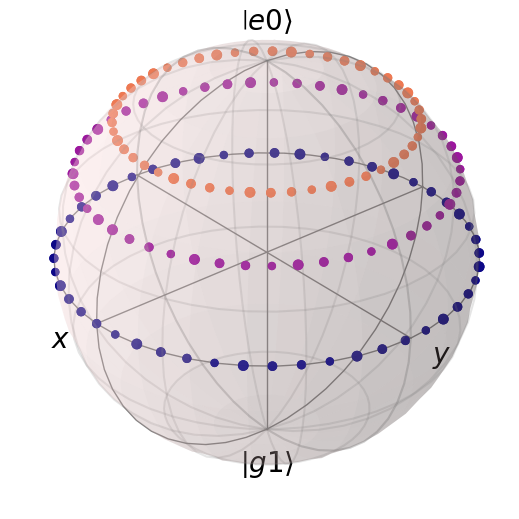
\includegraphics[width=\textwidth]{figuras/ch3/bloch berry.png}
        \caption{} 
        \label{fig3:bloch berry}
    \end{subfigure}
    \hfill
    \begin{subfigure}[h]{0.49\textwidth}
        \centering
        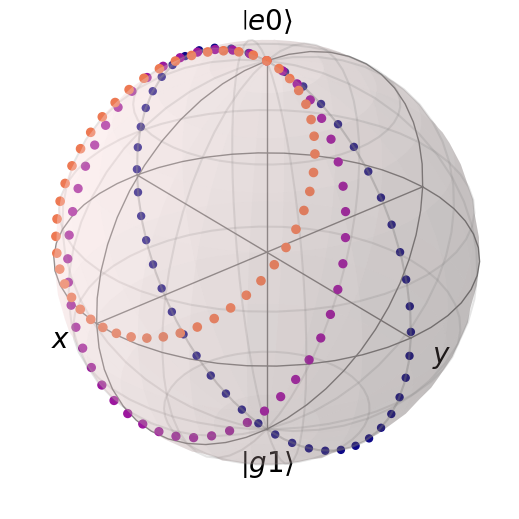
\includegraphics[width=\textwidth]{figuras/ch3/bloch cinematica.png}
        \caption{}
        \label{fig3:bloch cinematica}
    \end{subfigure}
    \caption{(\ref{sub@fig3:bloch berry}) Evolución de un autoestado $\ket{\psi_\pm(t)}$ bajo un campo de control que introduce cambios de fase. (\ref{sub@fig3:bloch cinematica}) Evolución de un estado genérico $\ket{e,n}$. Las curvas se corresponden con diferentes valores del detunning, que son $\Delta=0$ (azul), $\Delta=g$ (violeta) y $\Delta=2g$ (naranja).}
    \label{fig3:esfera de bloch jcm}
\end{figure}
La Figura \ref{fig3:bloch berry} muestra la evolución bajo el campo que introduce un corrimiento de fases utilizado para calcular la fase de Berry, los autoestados son los autoestados $R(\Omega)\ket{\psi_\pm^n}=e^{-i\Omega \hat n}\ket{\psi_\pm^n}$, entonces al variar $\Omega\in [0,2\pi]$ la trayectoria es simplemente un circulo paralelo al ecuador en la esfera de Bloch. En cambio, en el segundo caso, si preparamos el sistema inicialmente en el estado $\ket{e,n}$ y lo dejamos evolucionar por la acción del Hamiltoniano durante un tiempo, la trayectoria no consiste en círculos horizontales en la esfera, sino que parten del polo norte, que es el estado $\ket{e,n}$, y luego hace una trayectoria ovalada, para finalmente volver al punto inicial de partida a un tiempo $t=T$. La diferencia en el signo se explica a través de la transformación que nos lleva de una curva a la otra. Para esto, necesitamos de una rotación rígida, y una inversión de la parametrización, por su parte, esta última, introduce un signo negativo, cosa que se ve claramente en la Ec. (\ref{ec3:fg unitaria jcm}) al cambiar $t\rightarrow -t$.

\section{Medio no lineal}\label{sec3:medio kerr}
Para generalizar el resultado anterior, se le agrega un medio no lineal a la cavidad. Este medio se lo conoce como medio Kerr, y agrega un término en el Hamiltoniano de la cavidad Ec. (\ref{ec3:hamiltoniano inicial}):
\begin{equation}
    \hat H_C=\epsilon \hat n \rightarrow \hat H_C^{\text{Kerr}}=\epsilon \hat n (1+\frac{\chi}{\epsilon}\hat n),
\end{equation}
donde $\chi$ es el parámetro que caracteriza al medio de la cavidad Kerr. Este medio hace que la energía de la cavidad dependa de la cantidad de fotones de manera no lineal, donde $\chi$ es la frecuencia/energía característica de la dependencia cuadrática. Si se realiza nuevamente la RWA, se arriba a las mismas conclusiones sobre la forma del Hamiltoniano de la Ec. (\ref{ec3:hamiltoniano jcm}) y se obtiene
\begin{equation}
    \hat H=\frac{\Delta}{2}\hat \sigma_z+\chi \hat n^2+g(\hat a^\dagger \hat \sigma_-+\hat a \hat \sigma_+),
\end{equation}
y en forma matricial, en el subespacio de n excitaciones $\{\ket{gn},\ket{e,n-1}\}$:
\begin{equation}
    H^{(n)} = \begin{pmatrix}
        -\frac{\Delta}{2}+\chi n^2 & g \sqrt{n} \\
        g \sqrt{n} & \frac{\Delta}{2}+\chi (n-1)^2 
    \end{pmatrix}.
\end{equation}
Resolviendo, se obtiene que ahora los autovectores son
\begin{equation}\label{ec3:autoestado kerr}
    \ket{\psi_\pm^n}=\frac{1}{N_\pm} \left( (-\frac{\Delta}{2}+\chi(n-1/2)\mp\frac{\Omega_{n,\chi}}{2}) \ket{gn} + g\sqrt{n} \ket{e,n-1}  \right),
\end{equation}
donde $\Omega_{n,\chi}=\sqrt{(\chi(2n-1)-\Delta)^2+4g^2n}$, $N_\pm=\sqrt{(-\frac{\Delta}{2}+\chi(n-1/2)\mp\Omega_{n,\chi}/2)^2+g^2n}$, y las autoenergías son 
\begin{equation}\label{ec3:autoenergia kerr}
    E_\pm^n=\chi(n-\frac{1}{2})^2 +\frac{\chi}{4} \pm \frac{\Omega_{n,\chi}}{2}
\end{equation}
Se puede ver que el resultado con $\chi=0$ se reduce al caso visto anteriormente, que representa una cavidad con un medio lineal.

Si se quiere resolver la dinámica de este problema para un estado inicial cualquiera, lo que se tiene que hacer es desarrollar este estado inicial en función de los autoestados del problema. Entonces se tendría para un estado arbitrario con un número total de excitaciones definido, que suponemos igual a 1 por simplificación (la generalización es inmediata):
\begin{equation}
    \ket{\psi}(t)=U(t)(\braket{\psi_+^1}{\psi(0)}\ket{\psi_+^1}+\braket{\psi_-^1}{\psi(0)}\ket{\psi_-^1})=c_+e^{-iE_+t}\ket{\psi_+}+c_-e^{-iE_-t}\ket{\psi_-}.
\end{equation}
Resulta interesante notar que al sacar factor común la fase $e^{-iE_+t}$, la cantidad relevante sigue siendo $\Omega_{n,\chi}$, que es la frecuencia de Rabi para medios tipo Kerr. Por otro lado, el producto interno que da lugar a los coeficientes $c_\pm$ depende de $\chi$, por lo tanto las amplitudes de probabilidad de encontrar al estado temporalmente evolucionado en algún otro estado haciendo una medición proyectiva, depende de $\chi$. Concluyendo que el medio Kerr modifica las amplitudes de oscilación de las poblaciones del estado.

Entonces se analiza la relación entre $\pm \Omega_{n,\chi}/2$ y el detunning, teniendo en cuenta que ahora el medio puede tener $\chi \neq 0$. 

\begin{figure}[h]
    \centering
    \begin{subfigure}[h]{0.49\textwidth}
        \centering
        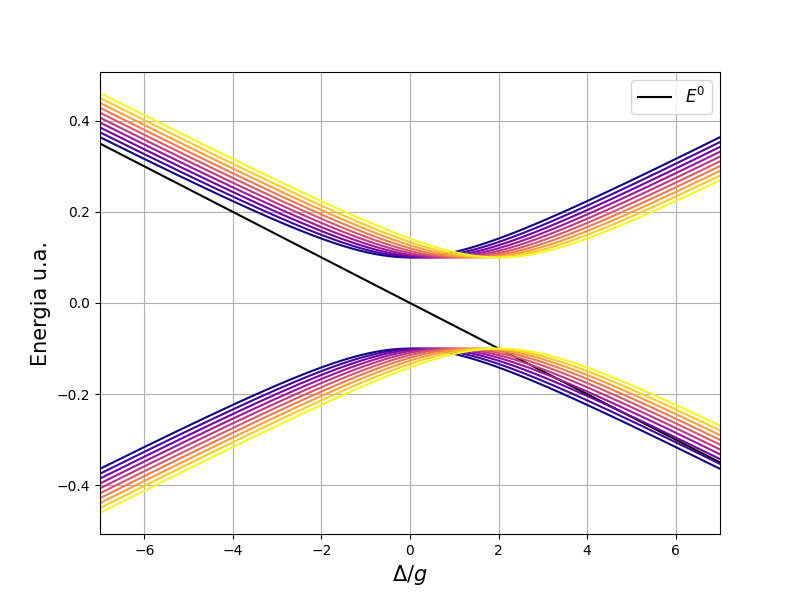
\includegraphics[width=\textwidth]{figuras/ch3/relacion energia detunning jcm simple kerr.png}
        \caption{}
        \label{fig3:relacion energia detunning kerr 1}
    \end{subfigure}
    \hfill
    \begin{subfigure}[h]{0.49\textwidth}
        \centering
        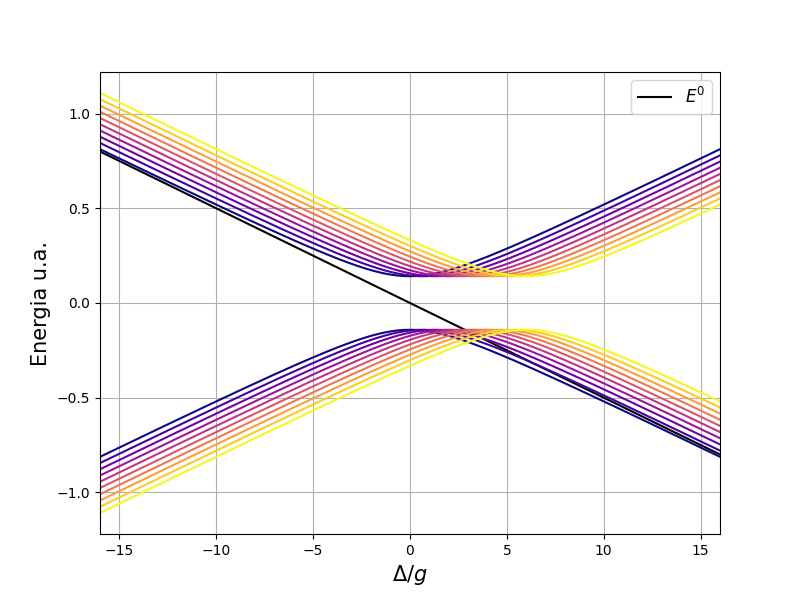
\includegraphics[width=\textwidth]{figuras/ch3/relacion energia detunning jcm simple kerr 2.png}
        \caption{}
        \label{fig3:relacion energia detunning kerr 2}
    \end{subfigure}
    \caption{Gráfico de la frecuencia de Rabi $\Omega_{N,\chi}$ en función del detunning $\Delta$ para (\ref{sub@fig3:relacion energia detunning kerr 1}) $N=1$ y (\ref{sub@fig3:relacion energia detunning kerr 2}) $N=2$.}
    \label{fig3:relacion energia detunning kerr}
\end{figure}

Se observa en la Figura \ref{fig3:relacion energia detunning kerr} como se modifica la frecuencia $\pm \Omega(N,\chi)$ para diferentes valores de $\chi$, donde en el panel (\ref{sub@fig3:relacion energia detunning kerr 1}) se muestran las energías para $N=1$ y en (\ref{sub@fig3:relacion energia detunning kerr 2}) para $N=2$, en función del detunning. En colores (de más oscuro a más claro) se aprecia cómo el aumento de $\chi \in [0,2g]$ afecta a las curvas: al aumentar $\chi$, las curvas se desplazan hacia la derecha en una cantidad $\chi(n-1/2)$. 

Este comportamiento se puede predecir mirando la forma de la autoenergía Ec. (\ref{ec3:autoenergia kerr}), ya que lo que estamos haciendo es desplazando la raíz mediante un cambio de variables $\Delta \rightarrow \Delta - \chi(2n-1)$. Este desplazamiento depende del número de excitaciones $n$. 
Dados dos valores diferentes de $\chi$ es de interés saber si al aumentar $\Delta$, aumentan o disminuyen las energías de los estados, por ejemplo, si se comparan dos casos, uno con $\chi_1=0$ y otro con $\chi_2=0.5g$, y dado un valor de detunning $\Delta=2g$, cuál de los dos casos tiene una mayor frecuencia?

Para esto se busca la intersección entre dos curvas con diferentes $\chi$, que llamamos $\chi_1$ y $\chi_2$, con $\chi_1<\chi_2$. Mediante un cálculo se obtiene que la intersección es para $\Delta=(2n-1)\frac{\chi_1+\chi_2}{2}$. Es decir, si $\Delta<(2n-1)\frac{\chi_1+\chi_2}{2}$ entonces la frecuencia de $\chi_2$ es mayor que la de $\chi_1$, y viceversa si $\Delta>(2n-1)\frac{\chi_1+\chi_2}{2}$.

Ahora, habiendo entendido esto, podemos ver que el efecto del medio es modificar la frecuencia y también la amplitud de la oscilación. En ambos casos, el mínimo de frecuencia y máximo de amplitud se alcanza cuando se cumple que 
\begin{equation}
    \Delta-\chi(2n-1)=0.
\end{equation}
Esta condición se da en el mínimo de energía, y por lo tanto es inmediato concluir que la frecuencia es mínima es este lugar. Además, cuando se cumple esta condición, los autoestados son autoestados de $\hat \sigma_x$, y los estados de la base evolucionan según
\begin{equation}
    \begin{aligned}
        \ket{gn(t)} &=\left[ A_g \left( \frac{e^{-iE_+t}}{N_+^2}+\frac{e^{-iE_-t}}{N_-^2}\right)-B_g\left( \frac{e^{-iE_+t}}{N_+^2}-\frac{e^{-iE_-t}}{N_-^2}\right) \right] \ket{gn} \\
        & + g\sqrt{n}\left[C_g\left( \frac{e^{-iE_+t}}{N_+^2}+\frac{e^{-iE_-t}}{N_-^2}\right)-D_g\left( \frac{e^{-iE_+t}}{N_+^2}-\frac{e^{-iE_-t}}{N_-^2}\right)\right]\ket{e,n-1},
    \end{aligned}
\end{equation}
con
\begin{equation*}
    \begin{aligned}
        A_g &= (-\Delta/2+\chi(n-1/2))^2+\Omega_{n,\chi}^2/4, \\
        B_g &= \Omega_{n,\chi}(-\Delta/2+\chi(n-1/2)), \\
        C_g & = g\sqrt{n}(-\Delta/2+\chi(n-1/2)), \\
        D_g & = g\sqrt{n}\Omega_{n,\chi}. 
    \end{aligned}
\end{equation*}
Para que las oscilaciones sean coherentes, se puede ver que cuando $\Delta-\chi(2n-1)=0$ las constantes $B_g=C_g=0$, $N_+=N_-=\sqrt{2}g\sqrt{n}$, y así el estado evoluciona como:
\begin{equation}
    \ket{gn(t)}=e^{-i(\chi(n-1/2)^2+\chi/4}\left[\cos(\Omega t/2)\ket{gn}-\sin(\Omega t/2)\ket{e,n-1}\right],
\end{equation}
y la evolución de $\ket{e,n-1(t)}$ debe ser el estado ortogonal. Si no se cumple la condición, entonces las oscilaciones no serán coherentes y su amplitud no será 1.

Una propiedad importante que se observa cuando se cumple la condición $\Delta-\chi(2n-1)=0$, es que el autoestado del Hamiltoniano es máximamente entrelazado (MES por sus siglas en inglés). Para ver esto se parte de la Ec. (\ref{ec3:autoestado kerr}) y la expresión para $\Omega_{n,\chi}$. Por un lado, es fácil ver que $\Omega_{n,\chi}=2g\sqrt{n}$ y se obtiene 
\begin{equation}
    \ket{\psi_\pm^n}=\frac{1}{\sqrt{2}}(\ket{gn}\mp \ket{e,n-1},
    \label{ec3:bell}
\end{equation}
que son estados de Bell. 


\section{Modelo de JC disipativo} 
\label{sec3:jcm disipativo}

Después del análisis de la fase geométrica acumulada por el sistema átomo-cavidad en la situación ideal de completo aislamiento, se aborda ahora el estudio para el escenario más realista en el que el mismo sistema se encuentra en interacción con un entorno, es decir, un modelo de JC disipativo.

Siguiendo la Ref. \cite{TesisViotti}, en esta sección se estudia en detalle la fase geométrica acumulada en un modelo de Jaynes-Cummings disipativo, como caso paradigmático dentro del campo de la electrodinámica en cavidades. Se considera que los principales mecanismos por los cuales el sistema “átomo + modo” interactúa con el entorno son el flujo de fotones a través de las paredes de la cavidad, y el continuo e incoherente bombeo del sistema de dos niveles, lo que conforma un escenario frecuente en electrodinámica de cavidades semiconductoras \cite{Khitrova2006}-\cite{DelValle2009}. 

Para poder modelar estos mecanismos, se emplea la ecuación maestra fenomenológica de Lindblad (ver Ap. \ref{ap_ecsmaestras})
\begin{equation}\label{ec3:lindblad}
\dot{\rho}(t) = -i [H, \rho(t)] + \frac{1}{2} \sum_\alpha \big( 2L_\alpha \rho(t) L_\alpha^{\dagger} - \{ L_\alpha^{\dagger}L_\alpha, \rho(t) \} \big),
\end{equation}
despreciando otros procesos con menor influencia en la dinámica como el desfasaje puro o el bombeo de fotones del entorno en la cavidad, donde además se ha considerado que el entorno se halla a temperatura cero. Los operadores de Lindblad

\begin{equation}
L_\gamma = \sqrt{\gamma} \ a,
\end{equation}
\begin{equation}
L_p = \sqrt{p} \ \sigma_+,
\end{equation}
representan la pérdida de fotones y el bombeo continuo e incoherente del átomo, respectivamente, con los parámetros $\gamma$ y $p$ denominados tasa de pérdida de fotones y amplitud del bombeo. 

El bombeo sobre el átomo es siempre secundario frente a la pérdida de fotones, lo cual nos da las relaciones $\frac{p}{g},\frac{p}{\gamma} \ll 1$, y la relación entre $\gamma$ y $g$ da lugar a dos regímenes que se diferencian con claridad \cite{Carmi1989}-\cite{Lodhal2015}. El régimen de acoplamiento fuerte (SC o Strong Coupling) aparece cuando la interacción átomo-cavidad es más fuerte que la disipación del entorno, es decir $\gamma /g <1$. En el caso contrario $\gamma/g>1$ estamos en el régimen de acoplamiento débil (WC o Weak Coupling). Para no generar confusiones, hay que destacar que, en general, cuando en la literatura se habla de acoplamientos fuertes y débiles, se refiere a la interacción entre las partes del mismo sistema, pero en este caso, se esta haciendo referencia a la interacción del sistema con el entorno \textit{en comparación} con la interacción interna del sistema.
\subsection{Solución y régimen de acoplamiento}\label{sec3:regimen acoplamiento}
En esta ocasión se resuelve el problema restringiéndose al subespacio donde el átomo puede estar en cualquiera de sus dos estados, y la cavidad tiene 1 o 2 fotones. En consecuencia, el problema se limita a un subespacio truncado cuya base son los estados $\{ \ket{0}=\ket{g,0} ; \ket{1}=\ket{e,0} ; \ket{2}=\ket{g,1} \}$. Desarrollar explícitamente el sistema de ecuaciones dadas por la ecuación de Lindblad Ec. (\ref{ec3:lindblad}), lleva a ecuaciones para los elementos $\rho_{0i}$ que quedan desacoplados de los demás:

\begin{equation}
    \begin{aligned}
        \dot \rho_{01} & =-\frac{p}{2} \rho_{01}+i\Delta\rho_{01}+ig\rho_{02} \\
        \dot \rho_{02} & =-\frac{p}{2} \rho_{02}-\gamma \rho_{02}+ig\rho_{01}
    \end{aligned}
\end{equation}
con lo cual, si inicialmente los elementos de matriz $\rho_{0i}(0)=0$, permanecerán así durante toda la evolución del sistema. Para hacer una analogía y comparar con el caso unitario, se estudia la condición inicial $\rho(0)=\ketbra{e,0}{e,0}$, de modo que la matriz $\rho(t)$ exhiba una estructura diagonal por bloques. El primer bloque de 1x1 representando al estado $\ket{0}$, y luego un bloque de 2x2 que describe la dinámica entre los estados $\ket{1}$ y $\ket{2}$. Las ecuaciones son

\begin{equation}
\begin{aligned}
\dot{\rho}_{00} &= -p \rho_{00} + \gamma \rho_{22} \\
\dot{\rho}_{11} &= -i g (\rho_{21} - \rho_{12}) + p \rho_{00} \\
\dot{\rho}_{22} &= -i g (\rho_{12} - \rho_{21}) - \gamma \rho_{22} \\
\dot{\rho}_{12} &= -i g (\rho_{22} - \rho_{11}) - i \Delta \rho_{12} - \frac{\gamma}{2} \rho_{12},
\end{aligned}
\end{equation}
se resuelven numéricamente para acceder al estado $\rho(t)$ a tiempo $t>0$. 

\begin{figure}[h]
    \centering
    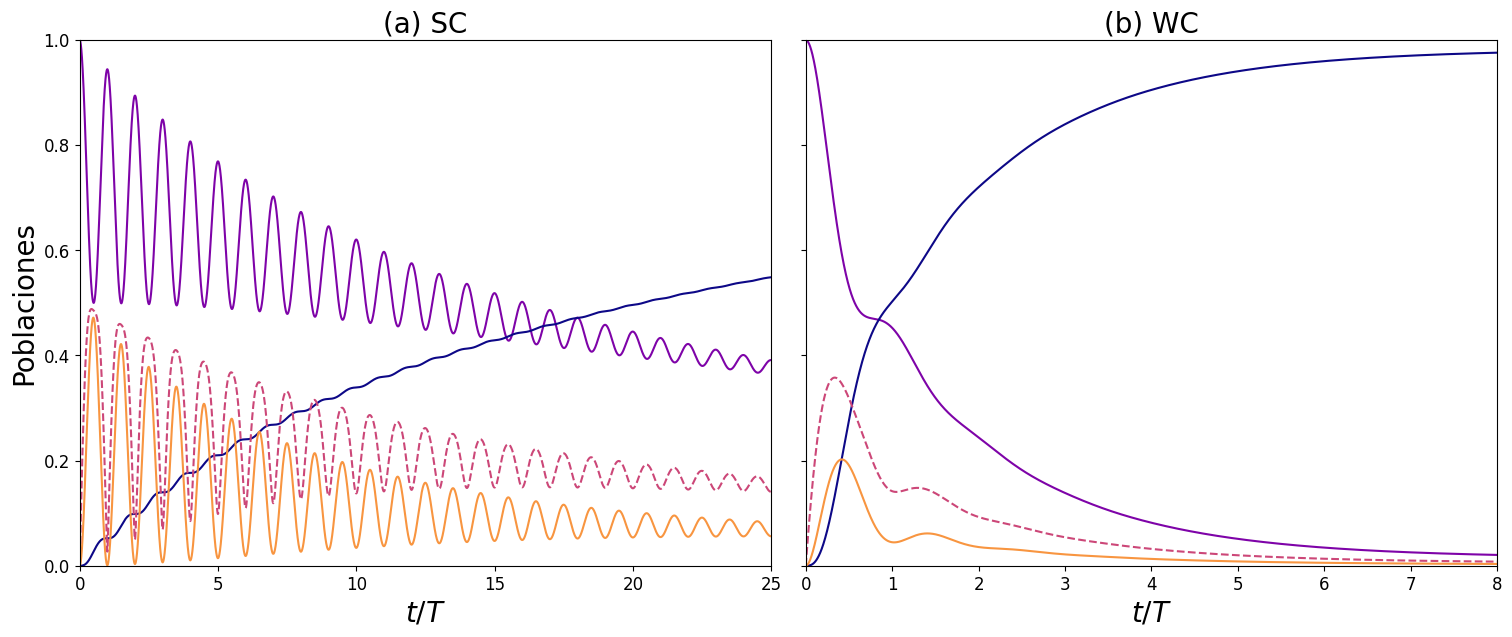
\includegraphics[width=\textwidth]{figuras/ch3/poblaciones sc vs wc.png}
    \caption{Solución numérica al sistema de ecuaciones dada por la ecuación de Lindblad para el estado inicial $\ket{e0}\bra{e0}$. Estos gráficos se realizaron con $\Delta=2g$; a la izquierda se observa el regimiento de WC con $\gamma=0.1g$, donde el sistema átomo-cavidad está débilmente acoplado con el entorno, y a la derecha el de SC con $\gamma=2g$, donde las poblaciones y coherencias decaen sin oscilar. Las lineas sólidas son las poblaciones de los estados, en azul para el estado $\ket{g0}$, en morado para $\ket{e0}$ y en amarillo $\ket{g1}$, y la línea rayada representa la coherencia entre los estados con N=1 ($\ket{e0}$ y $\ket{g1}$). }
    \label{fig3:poblaciones e0}
\end{figure}

En la Figura \ref{fig3:poblaciones e0}a, se muestra el régimen de SC, donde el acoplamiento entre el átomo y la cavidad es mayor al acoplamiento con el entorno, según la relación entre los parámetros $\gamma/g=0.1$, y en el panel \ref{fig3:poblaciones e0}b, se muestra el caso del WK. En el primer caso, tanto las poblaciones como las coherencias presentan oscilaciones coherentes antes de decaer por la influencia del entorno. En cambio, para el caso de WK, estas oscilaciones coherentes no están presentes y el sistema llega a su estado asintótico en tiempos muy cortos. Las características de la dinámica de cada régimen, influyen profundamente en el estudio de la fase geométrica, haciendo posible únicamente su utilización en el caso de Strong Coupling, donde la dinámica presenta oscilaciones coherentes durante varios ciclos, antes de decaer, haciendo del régimen de SC el único escenario conveniente para su estudio. Antes de fundamentar esta afirmación, se realiza un estudio poblacional en el caso de una cavidad con medio Kerr.
\begin{figure}[h]
    \centering
    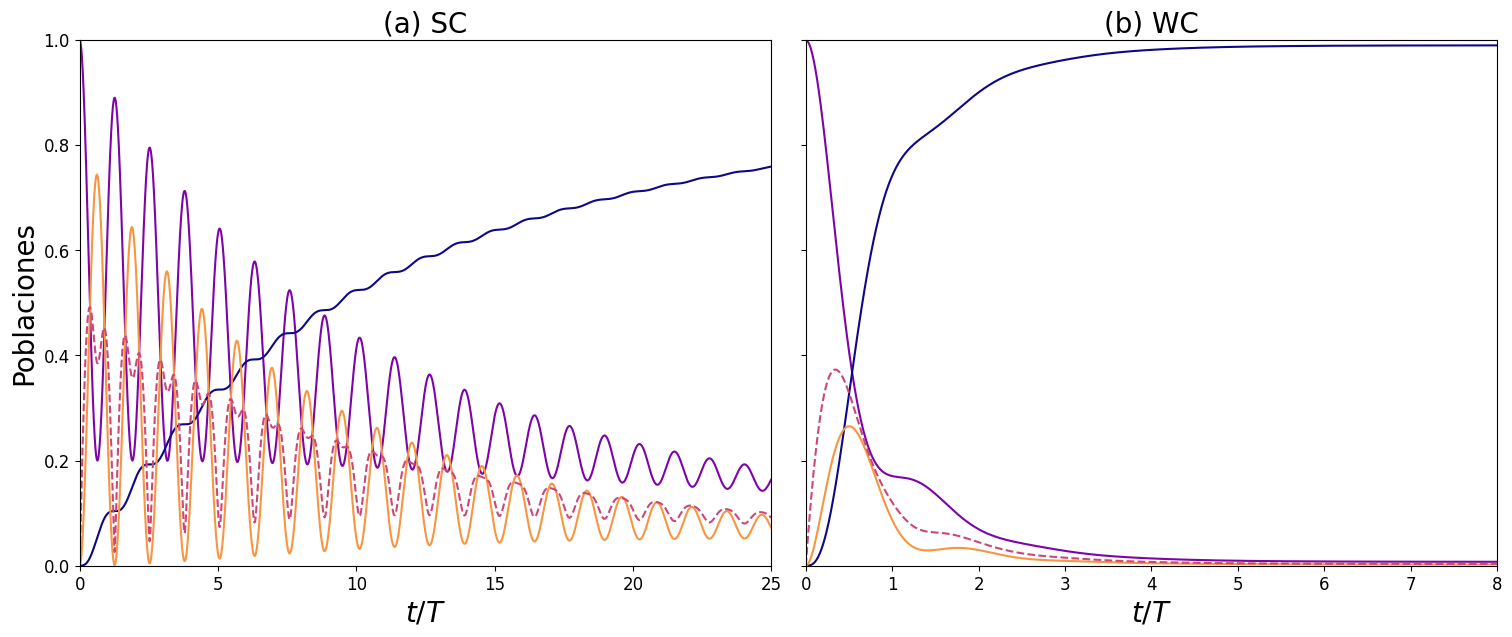
\includegraphics[width=\textwidth]{figuras/ch3/poblaciones kerr.png}
    \caption{Análisis poblacional para una cavidad con medio Kerr con $\chi=0.5g$. Para la simulación se utilizaron los mismos parámetros que en la Figura \ref{fig3:poblaciones e0}}
    \label{fig3:poblaciones kerr}
\end{figure}
Como se vio anteriormente, el efecto del medio Kerr sobre los autoestados y las autoenergías es, por un lado, desplazar los niveles de energía.
Si se comparan las Figuras \ref{fig3:poblaciones e0} con \ref{fig3:poblaciones kerr}, entonces se pueden observar dos diferencias. La primera es lo mencionado anteriormente; en el mismo tiempo, es decir entre $0\leq t/T \leq 25$, en el caso de $\chi=0$ se observan 25 oscilaciones, pero en el caso de $\chi=0.5g$ solo se observan 23 oscilaciones. Esto se debe a la condición que se encontró al final de la sección \ref{sec3:medio kerr}. En este caso se verifica que $\Delta=2g>(2n-1)\frac{\chi_1+\chi_2}{2}=\frac{g}{4}$, entonces la diferencia de energías entre los autoestados disminuye al aumentar $\chi$, y por lo tanto, las oscilaciones son más lentas para el caso de $\chi=0.5g$ en comparación con $\chi=0$.

\subsection{Fase geométrica en presencia de disipación}
\label{sec3:fg disipacion}
En esta sección se muestran algunos resultados conocidos acerca de la fase geométrica adquirida por el sistema, calculada siguiendo la definición de la Ec. (\ref{ec2:fg general}), y se analiza como esta se ve modificada con respecto del valor unitario por efecto del contacto con el entorno. Como el estado inicial es puro, la definición se reduce al caso particular descrito por la Ec. (\ref{ec2:fg general puro}).

Los autovalores y autovectores del operador densidad pueden escribirse formalmente  diagonalizando el subespacio de 2x2 de la matriz densidad:
\begin{equation}
    \rho(t)=\begin{pmatrix}
        \rho_{00} & 0 & 0 & 0 &\dots \\
        0 & \rho_{11} & \rho_{12} & 0 & \dots \\
        0 & \rho_{21} & \rho_{22} & 0 & \dots \\ 
        \vdots & 0 & 0 & \ddots & \dots 
    \end{pmatrix}
\end{equation}
donde se asume nuevamente una estructura diagonal por bloques, que se da cuando el estado inicial tiene un número definido de excitaciones, dando lugar a dos autovectores. De estos dos, es el de mayor energía el de interés para utilizar la definición de la fase geométrica Ec. (\ref{ec2:fg general puro})
\begin{equation}
    \ket{\psi_+}(t)=\frac{-(\rho_{22}-\epsilon_+)\ket{e,0}+\rho_{21}\ket{g,1}}{\left((\rho_{22}-\epsilon_+)^2+\rho_{21}\rho_{12} \right)^{1/2}},
\end{equation}
con $\epsilon_+=\frac{1}{2}(\rho_{11}+\rho_{22}+\sqrt{(\rho_{11}-\rho_{22})^2+4\rho_{12}\rho_{21}})$ el autovalor asociado. Recurriendo a este resultado, podemos escribir formalmente la fase geométrica en función de los elementos de matriz $\rho_{ij}(t)$ \cite{Viotti2022}:
\begin{equation}
    \phi_g(t)=\int_0^t dt' \frac{\Im \dot\rho_{21}\rho_{12}}{(\rho_{22}-\epsilon_+)^2+\rho_{12}\rho_{21}}.
\end{equation}

En general, esta fase diferirá de aquella acumulada en una evolución unitaria de forma que puede
escribirse, sin pérdida de generalidad, como $\phi_g=\phi_u+\delta\phi$, con $\delta\phi$ la diferencia entre la fase unitaria y
aquella modificada por la presencia del entorno. Caracterizar la corrección $\delta\phi$ permite relacionar este
objeto, perteneciente a la geometría misma del espacio de Hilbert, con los efectos de disipación y
decoherencia experimentados por el sistema, así como determinar bajo qué circunstancias $\delta\phi$ resulta
despreciable y se puede considerar que la fase geométrica es robusta (o no) al efecto del entorno.

\subsubsection{Dependencia con el régimen de acoplamiento}
En la Figura \ref{fig3:fg gamma} se muestra la fase geométrica acumulada en función del tiempo adimensionalizado por un tiempo característico $T=\frac{2\pi}{\Omega_{n,\chi}}$, para el estado inicial puro $\ket{e,0}$, comparando 4 casos para la relación $\gamma/g$ pertenecientes al régimen de SC. Como referencia, además, se muestra la fase geométrica unitaria.
\begin{figure}[H]
    \begin{minipage}[c]{0.67\textwidth}
        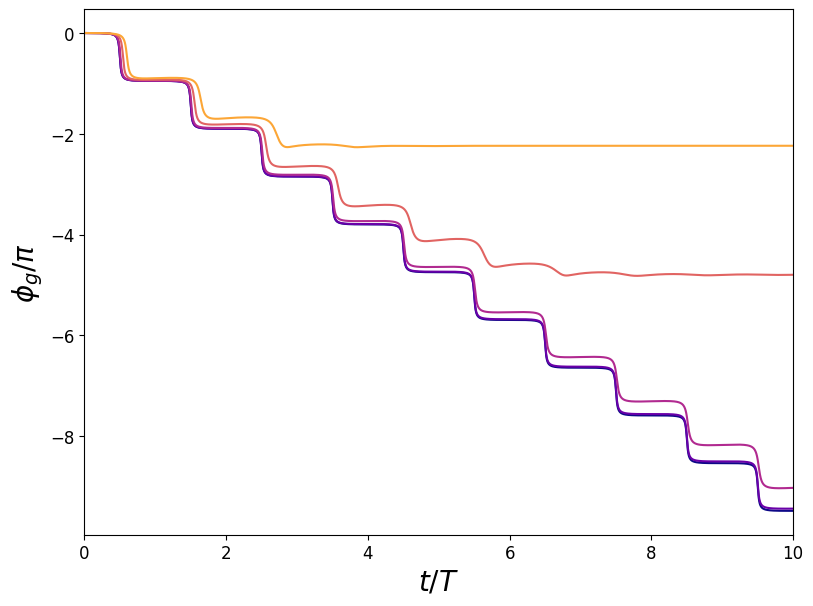
\includegraphics[width=\textwidth]{figuras/ch3/fg gamma.png}
      \end{minipage}\hfill
      \begin{minipage}[c]{0.3\textwidth}
        \caption{
            Fase geométrica acumulada por un sistema con un detunning $\Delta=0.1g$, para diferentes valores característicos del entorno. En todos los casos la tasa de bombeo es $p=0.005g$, y se muestran diferentes valores para $\gamma$, partiendo de $\gamma=0$ perteneciente a la línea azul oscuro que es el caso unitario, y para $\gamma=0.01g$,$\gamma=0.1g$,$\gamma=0.5g$ y $\gamma=g$, correspondientes a las lineas violeta, rosa, naranja y amarilla.
        } \label{fig3:fg gamma}
      \end{minipage}
\end{figure}
Al aumentar la interacción con el entrono, aumenta la diferencia $\delta \phi$ entre la fase acumulada con aquella correspondiente al caso unitario. Sin embargo, si el valor aumenta demasiado, la pérdida de coherencia detiene el movimiento del estado y consecuentemente la acumulación de fase. Por esto es que el estudio sobre la fase geométrica debe ser en el régimen de SC, ya que si la relación $\gamma/g\gg 1$, la fase dejará de acumularse luego de un período muy corto de tiempo.


\subsubsection{Dependencia con el detunning}
Ya que las amplitudes de los estados y las frecuencias de oscilación dependen de los parámetros del problema, entonces la curva que describe el estado en el espacio de rayos dependerá también de estos, heredando así la fase geométrica una dependencia con los parámetros. Manteniendo las características del entorno iguales, se estudia la dependencia de la fase geométrica con el detunning $\Delta$. En la Figura \ref{fig3:fg detunning} se observa que conforme se aumenta el detunning átomo-cavidad, la fase acumulada es menor (en valor absoluto) y se suaviza.
\begin{figure}[h]
    \begin{minipage}[c]{0.67\textwidth}
        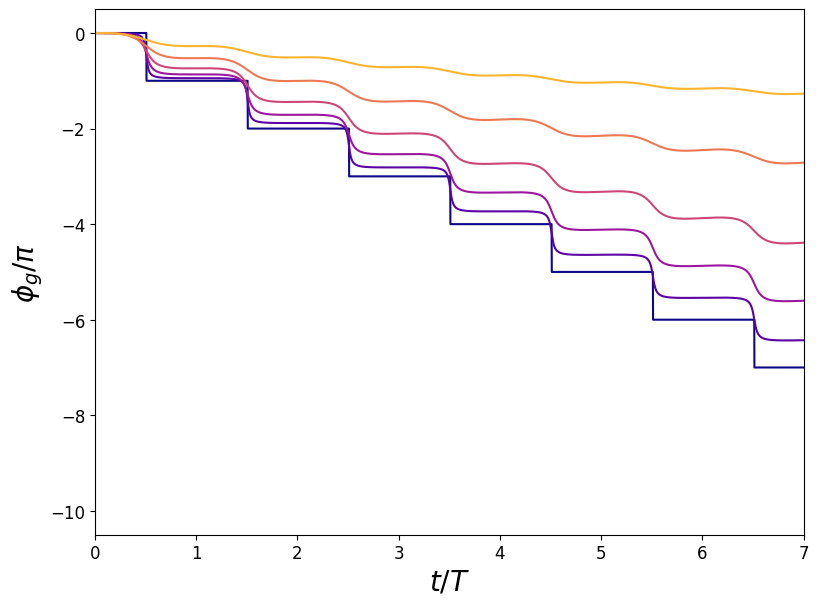
\includegraphics[width=\textwidth]{figuras/ch3/fg detunning.png}
    \end{minipage}\hfill
    \begin{minipage}[c]{0.3\textwidth}
    \caption{Fase geométrica acumulada por el estado inicial para diferentes valores del detunning. El entorno esta caracterizado por una tasa de bombeo $p=0.005g$ y una tasa de pérdidas $\gamma=0.1g$. Los valores de $\Delta$ varían entre $0$ (línea azul) y $2.5g$ (línea amarilla).}
    \label{fig3:fg detunning}
  \end{minipage}
\end{figure}

Como se discutió anteriormente, la fase geométrica en presencia del entorno se puede descomponer en la parte unitaria $\phi_u$ dada por la Ec. (\ref{ec2:fg cinematica unitaria}), más una corrección $\delta\phi$ que refleja la desviación introducida por el entorno. La dependencia de la componente unitaria en $\Delta/g$ esta explícita en la Ec. (\ref{ec3:fg unitaria jcm}). Surge entonces la pregunta de la dependencia del término $\delta\phi$ con respecto a los parámetros del problema, o si toda la dependencia se encuentra contenida en la parte unitaria $\phi_u$. Para tratar con esta pregunta se analiza la corrección $\delta\phi$ en un instante dado (que se elije y se mantiene fijo), observándola como función del valor de $\Delta/g$. El resultado se presenta en la Figura \ref{fig3:robustez 0}, en el cual se contrasta además esta dependencia para tres entornos caracterizados por distintos valores de tasa de perdida de fotones $\gamma$.
\begin{figure}[h]
    \begin{minipage}[c]{0.67\textwidth}
        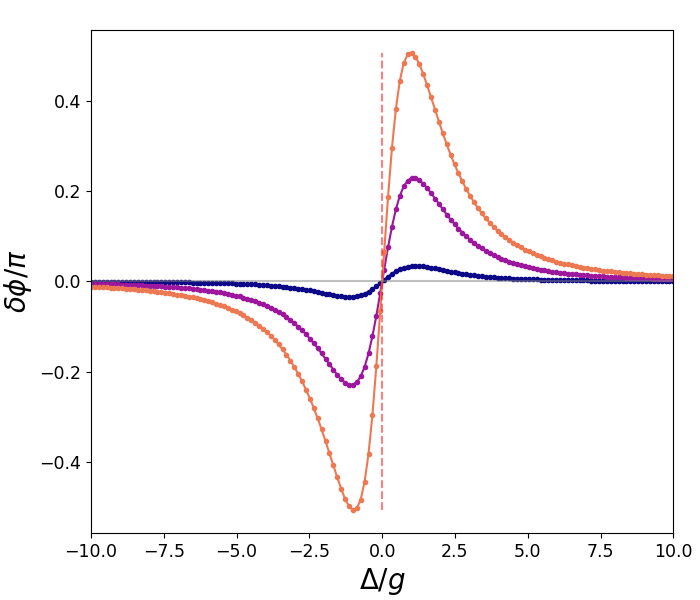
\includegraphics[width=\textwidth]{figuras/ch3/robustez.png}
    \end{minipage}\hfill
    \begin{minipage}[c]{0.3\textwidth}
    \caption{Diferencia de fase geométrica acumulada en función del detunning átomo-cavidad $\Delta$, para $\chi=0$ y para 3 medios distintos, cuyas tasas de perdida de fotones son $\gamma/g=0.01g,0.1g,0.25g$, asignadas a los colores violeta oscuro, morado y amarillo respectivamente.}
    \label{fig3:robustez 0}
  \end{minipage}
\end{figure}
Puede verse que la corrección en efecto depende del valor del detunning $\Delta/g$, y dos aspectos resaltan. En primer lugar, la corrección se anula, en todos los casos considerados, cuando se satisface la condición de resonancia $\Delta=0$. Este hecho resulta prometedor, insinuando que en este caso la fase geométrica $\phi_g$ resultaría robusta a los efectos de un entorno en el régimen de SC. La otra característica de la corrección $\delta\phi$ que se revela en la Figura \ref{fig3:robustez 0} es la no-monotonicidad de la corrección como función de $\Delta/g$, que exhibe un extremo para un valor $\Delta/g$ que depende débilmente tanto en las constantes $\gamma/g$ y $p/g$ que caracterizan el entorno como en el instante $t$ en el que se realiza la observación. De esta forma la Figura \ref{fig3:robustez 0} despierta un interés doble, ya que permite identificar: (i) las condiciones en las cuales el efecto del entorno sobre la fase geométrica es mayor, acercando la posibilidad de una detección experimental y, (ii) las condiciones que mitigan, permitiendo ignorarlo, este efecto o incluso que lo eliminan por completo.

\subsubsection{Dependencia con el medio Kerr}

Ahora se considera la dependencia con el medio Kerr. Al estudiar los efectos del detunning, se consideró que la cavidad era lineal, es decir $\chi=0$. Es ahora el objeto de estudio ver cómo se modifican la fase geométrica y los resultados obtenidos para el detunning al considerar un medio Kerr. En primer lugar, se muestra la dependencia de la fase geométrica acumulada para diferentes valores de $\chi/g$, considerando un entorno idéntico en todos los casos, con un valor fijo del detunning.

\begin{figure}[H]
    \centering
    \begin{subfigure}{0.49\textwidth}
        \centering
        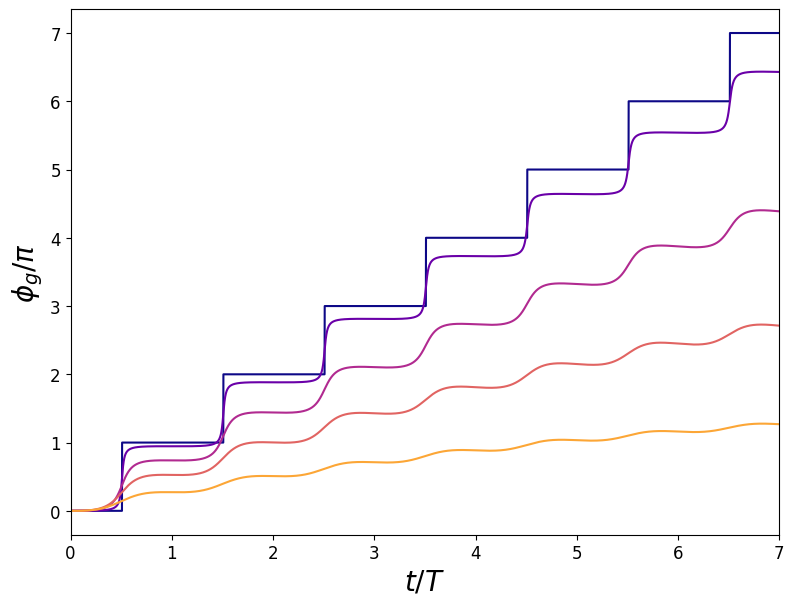
\includegraphics[width=\textwidth]{figuras/ch3/fg kerr.png}
        \caption{}
        \label{fig3:fg kerr 1}
    \end{subfigure}
    \hfill
    \begin{subfigure}{0.49\textwidth}
        \centering
        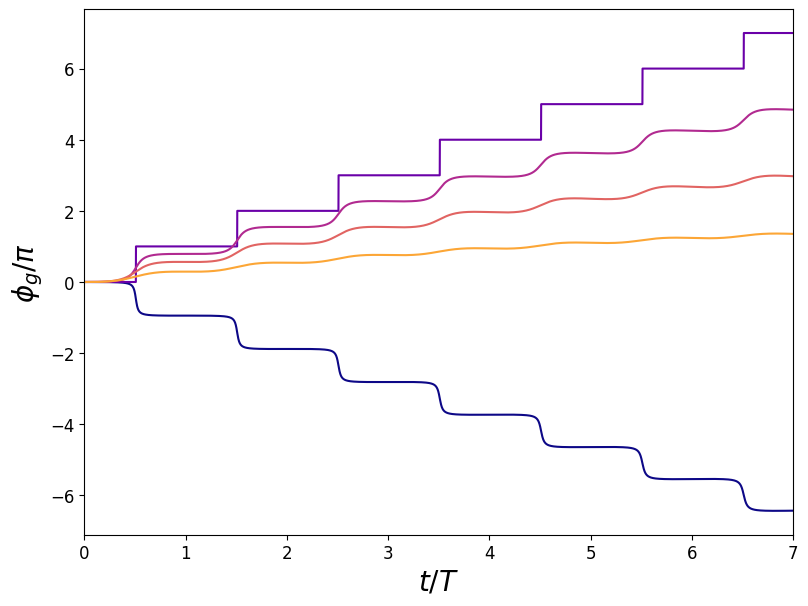
\includegraphics[width=\textwidth]{figuras/ch3/fg kerr d=0.1g.png}
        \caption{}
        \label{fig3:fg kerr 2}
    \end{subfigure}
    \caption{Dependencia de la fase geométrica acumulada para diferentes valores del medio Kerr dados por $\chi=0$, $0.1g$, $0.5g$, $g$ y $2g$ representados por colores partiendo del mas oscuro al mas claro, y un valor fijo del detunning: (\ref{sub@fig3:fg kerr 1}) $\Delta=0$ y (\ref{sub@fig3:fg kerr 2}) $\Delta=0.1g$}
\end{figure}
En la Figura \ref{fig3:fg kerr 1} se observa el efecto del medio sobre la fase geométrica acumulada, donde la línea azul oscuro, correspondiente al caso $\chi=0$ se corresponde con el caso robusto en donde tenemos una acumulación por escalones. Al comparar con la fase correspondiente a $\Delta=\chi=0$ de la Figura \ref{fig3:fg detunning} hay una diferencia notable, y es que en esta la fase acumulada es negativa, mientras que en la Figura \ref{fig3:fg kerr 1} es positiva. Esta discrepancia entre simulaciones para los mismos parámetros se debe a algo numérico. 

Al aumentar el parámetro $\chi$, similarmente al caso del detunning, la fase acumulada es menor y se suaviza. Este comportamiento es algo esperable, ya que en la ecuación para la energía el detunning $\Delta$ y el medio $\chi$ están casi en igualdad de condiciones, en el sentido que la dependencia funcional de la energía en estos parámetros es igual.
En la Figura \ref{fig3:fg kerr 2}, donde se considero un valor de $\Delta=0.1g$, se aprecia como el caso de $\chi=0$ (línea azul oscuro), ya no pertenece al caso robusto, sino que esta situación se recupera cuando $\chi=0.1g=\Delta$ (línea morada). Al seguir aumentando $\chi$ el comportamiento es igual que antes, la fase se acumula mas lentamente y los escalones se suavizan. 
Este resultado insinúa que para la fase geométrica, el medio y el detunning también están en igualdad de condiciones. Dos preguntas son pertinentes para confirmar esta intuición. En primer lugar, para corroborar la dependencia de la fase geométrica en el parámetro $\chi$, hay que realizar el estudio de la dependencia de la diferencia de fases geométricas $\delta\phi$ al igual que en el caso del detunning. En segundo lugar, se quiere ver como cambia la robustez en función del detunning si cambiamos el medio. Por lo tanto se repetirá el estudio en función del detunning, pero para diferentes valores de $\chi$.
\begin{figure}[h]
    \begin{minipage}[c]{0.67\textwidth}
        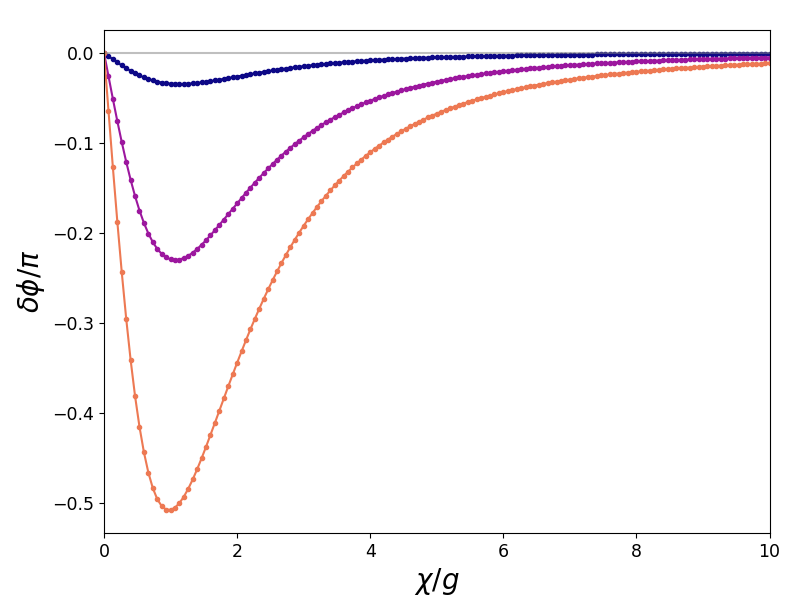
\includegraphics[width=\textwidth]{figuras/ch3/robustez kerr.png}
    \end{minipage}\hfill
    \begin{minipage}[c]{0.3\textwidth}
    \caption{Diferencia de fase geométrica acumulada en función del parámetro del medio $\chi$, para $\Delta=0$ y para 3 medios distintos, cuyas tasas de perdida de fotones son $\gamma/g=0.01g,0.1g,0.25g$, asignadas a los colores violeta oscuro, morado y amarillo respectivamente.}
    \label{fig3:robustez kerr}
  \end{minipage}
\end{figure}

En la Figura \ref{fig3:robustez kerr} se observa la dependencia de la diferencia en la fase geométrica acumulada en función del parámetro del medio $\chi$. El comportamiento es el mismo que con el detunning: la diferencia se anula para $\chi=0$, que coincide con el caso de robustez $\Delta=0$. La diferencia es que ahora la fase acumulada es negativa, pero solo es una reflexión con respecto al caso anterior. Esto se debe a que el detunning $\Delta$ y el parámetro del medio $\chi$, tienen signos diferentes en todas las expresiones vistas anteriormente y la fase hereda este signo, conservando los demás comportamientos. En este caso también hay un máximo no trivial que depende suavemente de los parámetros $\gamma/g$ y $p/g$, consecuentemente la dependencia en la fase geométrica en este parámetro no es trivial, y al igual que en el caso del detunning, es no-monótona, por lo tanto tiene las mismas implicaciones que en el caso anterior. Resulta interesante estudiar como se comportan ambos parámetros en conjunto. Se espera que, por los comportamiento observados hasta ahora, en realidad la dependencia general sea en $\Delta-\chi(2n-1)$, por lo tanto, se realiza nuevamente el estudio de robustez en función del detunning, para un valor $\chi/g=1$, que se observa en la Figura \ref{fig3:robustez mixta}.
\begin{figure}[h]
    \begin{minipage}[c]{0.67\textwidth}
        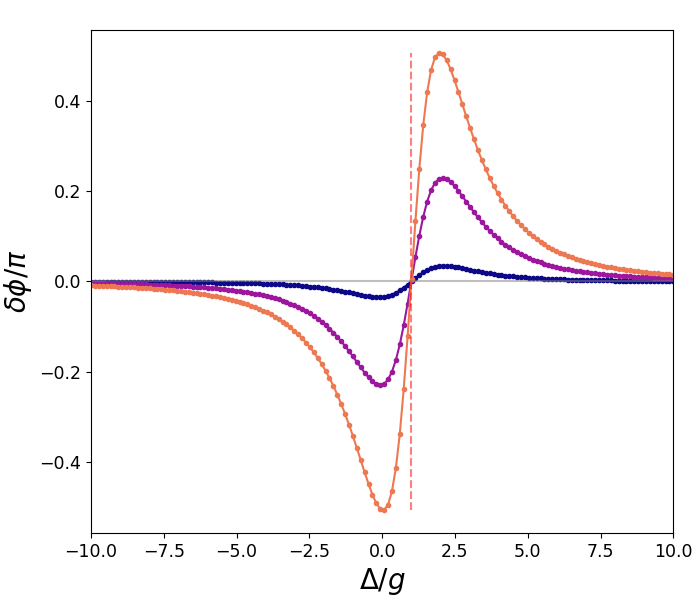
\includegraphics[width=\textwidth]{figuras/ch3/robustez x=g.png}
    \end{minipage}\hfill
    \begin{minipage}[c]{0.3\textwidth}
    \caption{Diferencia de fase geométrica acumulada en función del detunning átomo-cavidad $\Delta$, para $\chi=g$ y para 3 medios distintos, cuyas tasas de perdida de fotones son $\gamma/g=0.01g,0.1g,0.25g$, asignadas a los colores violeta oscuro, morado y amarillo respectivamente. Se observa como la condición de robustez se alcanza para $\Delta/g=\chi/g=1$.}
    \label{fig3:robustez mixta}
  \end{minipage}
\end{figure}
Se observa ahora una simetría al rededor de $\Delta=\chi=g$, donde se encuentra el cero de esta relación. Esto es lo que se esperaba, ya que en este caso de $n=1$, la dependencia será en $\Delta-\chi(2n-1) \implies \Delta-\chi$, es decir, si en el caso de $\chi=0$ la robustez se da para $\Delta=0$, la predicción es que los demás casos robustos se den en general cuando se cumple la relación 
\begin{equation}\label{ec3:condicion robuestez 1 atomo}
        \Delta-\chi(2n-1)=0
\end{equation}
comportamiento que se observa en la Figura \ref{fig3:robustez mixta}. 

Además, cuando se cumple esta condición, los autoestados del problema son los estados máximamente entrelazados de Bell, al igual que en el caso de medio lineal Ec. (\ref{ec3:bell}).
\subsubsection{Robustez de la fase geométrica en el caso resonante}

En esta sección se discute la razón detrás de la robustez en los casos estudiados anteriormente. 

Como se ha mencionado, las Figuras \ref{fig3:robustez 0}, \ref{fig3:robustez kerr} y \ref{fig3:robustez mixta}, muestran el resultado notable de que la diferencia $\delta\phi$ entre la fase geométrica acumulada en una hipotética evolución unitaria y la fase geométrica acumulada por el sistema abierto se anula cuando se satisface la condición de resonancia $\Delta = 0$ cuando el medio es lineal, y una segunda condición que llamaremos \textbf{condición de robustez}: $\Delta-\chi(2n-1)=0$ en el caso de considerar un medio tipo Kerr. La condición de robustez claramente incluye a la primera y es más general. El resultado sugiere que la fase geométrica es robusta a los efectos del entorno en este caso. Esta robustez puede estudiarse y explicarse en términos geométricos analizando la evolución del estado $\rho(t)$ del sistema átomo-modo y se vincula con el salto en $\pi$ que exhibe la fase geométrica unitaria $\phi_u$ del sistema resonante, cuyo estado describe un círculo máximo de la esfera de Bloch.

Para explicar el salto en $\pi$ de la fase unitaria es necesario recordar, como fue desarrollado en las secciones \ref{sec2:adiabatico} y \ref{sec2:no ciclico}, que la fase geométrica asociada a una trayectoria unitaria no-cíclica puede entenderse como la fase geométrica asociada a una curva cerrada específica: aquella construida a partir de la trayectoria abierta original, luego cerrada mediante una curva geodésica que conecte sus extremos. Esta interpretación permite explicar un salto abrupto en $\pi$ que muestra la fase geométrica acumulada en la evolución del sistema cuando el estado recorre un meridiano de la esfera de Bloch. Debido a que las geodésicas de la esfera de Bloch son, precisamente, sus círculos máximos, cuando la evolución recorre uno de éstos sin alcanzar a transitar la mitad de su longitud, la curva geodésica que debe considerarse coincide con la trayectoria de forma que la curva cerrada retorna sobre si misma acumulando fase geométrica nula. Por el contrario, si la trayectoria descrita por el estado supera la mitad del círculo máximo, la geodésica que une sus extremos lo completa encerrando un área de $2\pi$ que corresponde a una fase geométrica $\phi_u=\pi$.

Para el caso de un sistema en interacción con el entorno, la identidad formal entre la ecuación (\ref{ec2:fg general puro}) y la fase geométrica unitaria para el autoestado $\ket{\psi_+(t)}$ de la matriz densidad demanda el estudio de la curva descrita en la esfera de Bloch por (la proyección de) $\ket{\psi_+(t)}$. Lo que se observa es que para el caso robusto $\ket{\psi_+(t)}$ recorre una trayectoria que se superpone con aquella descrita por su análogo unitario pero que por efecto del entorno resulta de menor longitud (para un intervalo temporal idéntico). En un período $t \in [0, T]$ de evolución, entonces, el rayo asociado al estado $\ket{\psi(t)}$ retorna al punto inicial describiendo una trayectoria cíclica, mientras que aquél asociado a $\ket{\psi_+(t)}$ describe una curva abierta. Sin embargo, esto no afecta el valor obtenido para la fase geométrica que resulta $\phi_g=\pi$ siempre que el rayo recorra más de la mitad del círculo máximo. En consecuencia, siempre y cuando los efectos disipativos no sean lo suficientemente destructivos como para impedir que el autoestado supere el polo opuesto en un intervalo $t' \in [0, T]$, la fase geométrica acumulada en un período no se verá afectada. En este sentido, el caso robusto resulta entonces la situación ideal para realizar detecciones experimentales o implementar aplicaciones tecnológicas que requieran un escenario en que se puedan despreciar los efectos del entorno.

\section{Conclusiones}
En este capítulo se estudió en detalle la dinámica, y los efectos del medio Kerr sobre el modelo de JC. También se consideró el efecto del entorno sobre las poblaciones y en particular, el efecto que éste tiene sobre la fase geométrica. Se logró extender el entendimiento de la condición de robustez de la fase geométrica encontrado en la Ref. \cite{Viotti2022} para englobar el caso más general de un medio no lineal de tipo Kerr, donde el resultado importante es que en general, la robustez se da para $\Delta-\chi(2n-1)=0$.